\documentclass[10pt]{article}
\usepackage{amsmath}
\usepackage{amssymb}
\usepackage{graphicx}
\usepackage{epstopdf}
\usepackage{inputenc}
\usepackage{geometry}
\usepackage{pdfpages}


\title{Theme: NMT Carpool Project \\ Group Name: Algo}
\author{Julian Garcia \\ Saugat Sharma}

\begin{document}

\maketitle

\section{Background}
There's a fair amount of Techies who don’t have vehicles of their own. Many students have to rely solely on their friends and luck to get rides to places they need to be, many of whom are trying to get to ABQ to visit family or friends, there are even some out-of-state students who have hope that one of their friends will have the time to drive them to the airport to get home during school breaks.  There are also even students who live off campus, in Socorro, that struggle to get to class on time without a reliable vehicle. On the flip side of this, there are students who are commuting every day from ABQ to get to campus, and they'd most likely appreciate the opportunity to save money on gas in exchange for offering some other students a ride. All in all, this service could really benefit our community and could even help off campus students develop new friendships around campus. This could also help with Tech’s constant lack of parking spots if students with rides of their own decide to carpool with someone else, and in that case it'd also somewhat help us be a greener campus by reducing some carbon emissions.

\section{Website Analysis}

\subsection{5 Similar Websites}
The 5 websites we chose are as follows:
\begin{itemize}
  \item https://www.uber.com/
  \item http://www.bandwagon.io/
  \item https://www.v3cube.com/university-ride-sharing-clone/
  \item https://www.zimride.com/
  \item https://carpooltoschool.com/
\end{itemize}
Most of the websites we found mainly rely on apps to implement their features, which makes sense as users are more likely to use ride-ordering services when the only device they have on them is their phone. Most of the features of each site are very similar, clearly emulating each other.
\subsection{Desired Website Functions}
The functions we aim to implement and how we derived them are as follows: 
\begin{itemize}
  \item v3cube's service seemed the most interesting/relevant to our site. They have an almost pyramid-scheme like setup where there's a driver, passenger, and admin. The passenger searches for a ride, the driver lists how many seats they have and what fare they want, once the two reach an agreement, the admin makes sure the ride went well, and takes a cut of whatever the driver earned. We'd mainly like to implement the agreement system, and the driver's listings for seats as well as their desired price.
  \item Uber's ride search feature, you can find a ride on Uber by location and destination. Though we'd limit the scope of what locations you can request from. Ideally we'd be able to show the nearest ride available.
  \item Carpool World has a social media-ish profile setup, where users can set profile pictures, describe their typical routes, and give a description of how flexible they are as a driver. We'd like to emulate that profile setup, with additional sections about their major at Tech, whether they're an undergrad or graduate, and an expanded description of what they're like as a person. Uber also does this more expanded profile management.
  \item We'd like to authenticate our user-base by only allowing people with authenticated @student.nmt.edu or other nmt associated emails to join the site. Zimride also tries to implement this kind've authentication, though they do it through creating networks especially for each university they serve.
  \item Unlike these example websites, our site wouldn't require any payment throughout the whole process. The idea would mainly be to allow people who need to carpool to meet other students who are willing to carpool. Any type of payment would be agreed upon between the users individually, our site would just allow them to meet and talk. Which means we'll either have a messaging service as part of the site, or would allow students to share emails on their profile.
  \item Each of the services we've looked at all have a responsive map, that centers around the users given location. We'd try to use an api to implement this, and we'd display a map of NM showing all the routes students are taking/want to take.
  \item Car Pool to School has a calendar feature to handle all reminders and plans for carpool rides, we'd like to emulate this, ideally we'd be able to implement a calendar setup that could send reminders to a students email, so ideally students wouldn't be left forgotten after a set ride.
\end{itemize}
\newpage
\subsection{Progress Table}

\begin{table}[h!]
\resizebox{\columnwidth}{!}{\begin{tabular}{|l|l|l|l|l|l|l|}
\hline
 & Our Website & Uber & Bandwagon & v3cube & Zimride & Car Pool to School \\ \hline
Ride Search & v & v & x & v & x & v \\ \hline
Social Media Profiles & v & v & x & v & x & v \\ \hline
NMT authentication & v & x & x & x & x & x \\ \hline
Messaging Service & v & v & x & v & x & v \\ \hline
Interactive Map & v & v & x & o & v & v \\ \hline
Scheduling/Calendar & v & v & x & x & v & v \\ \hline
Flexible Agreement System & v & x & x & v & x & x \\ \hline
\end{tabular}}
\end{table}

\section{StoryBoard}
\subsection{Two users}
The two main users of this website would be NMT students/faculty who need a ride to NMT, and NMT students/faculty who can offer a ride to NMT. The notes in red on our storyboard will help explain how each would experience the website.

\subsection{Storyboard Desktop}
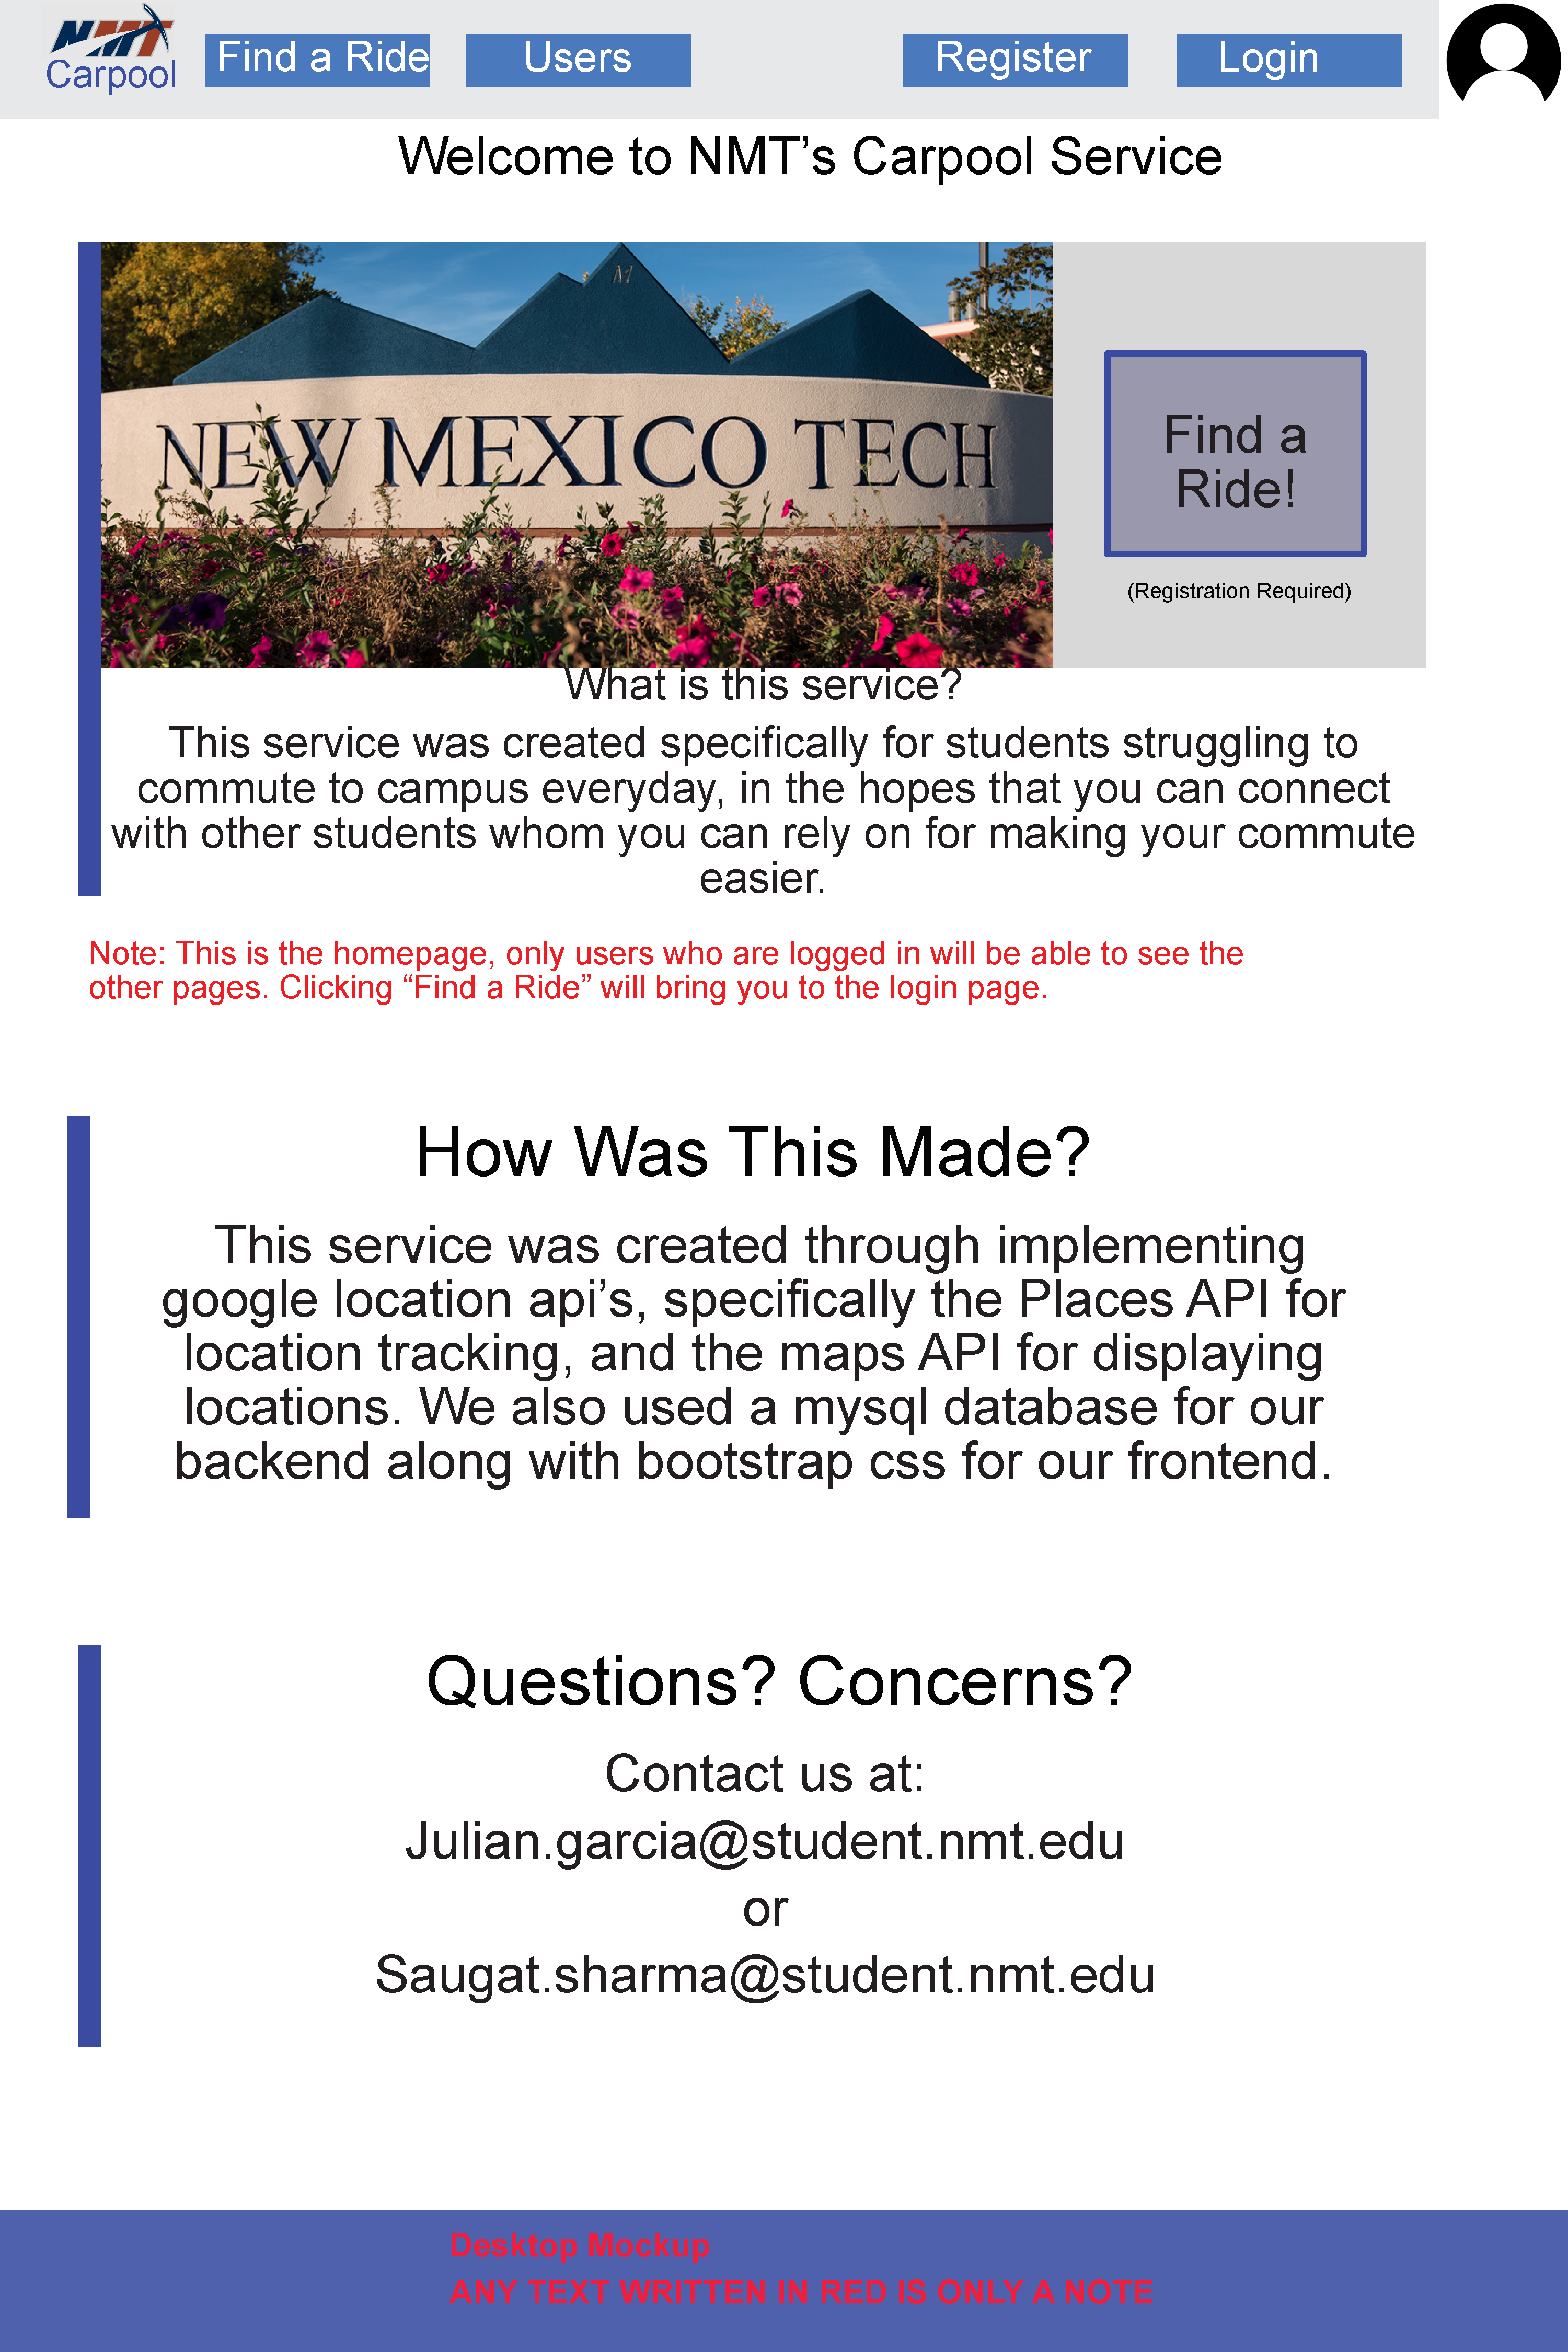
\includepdf[pages={-}]{MockupComplete.pdf}

\subsection{Storyboard Mobile}
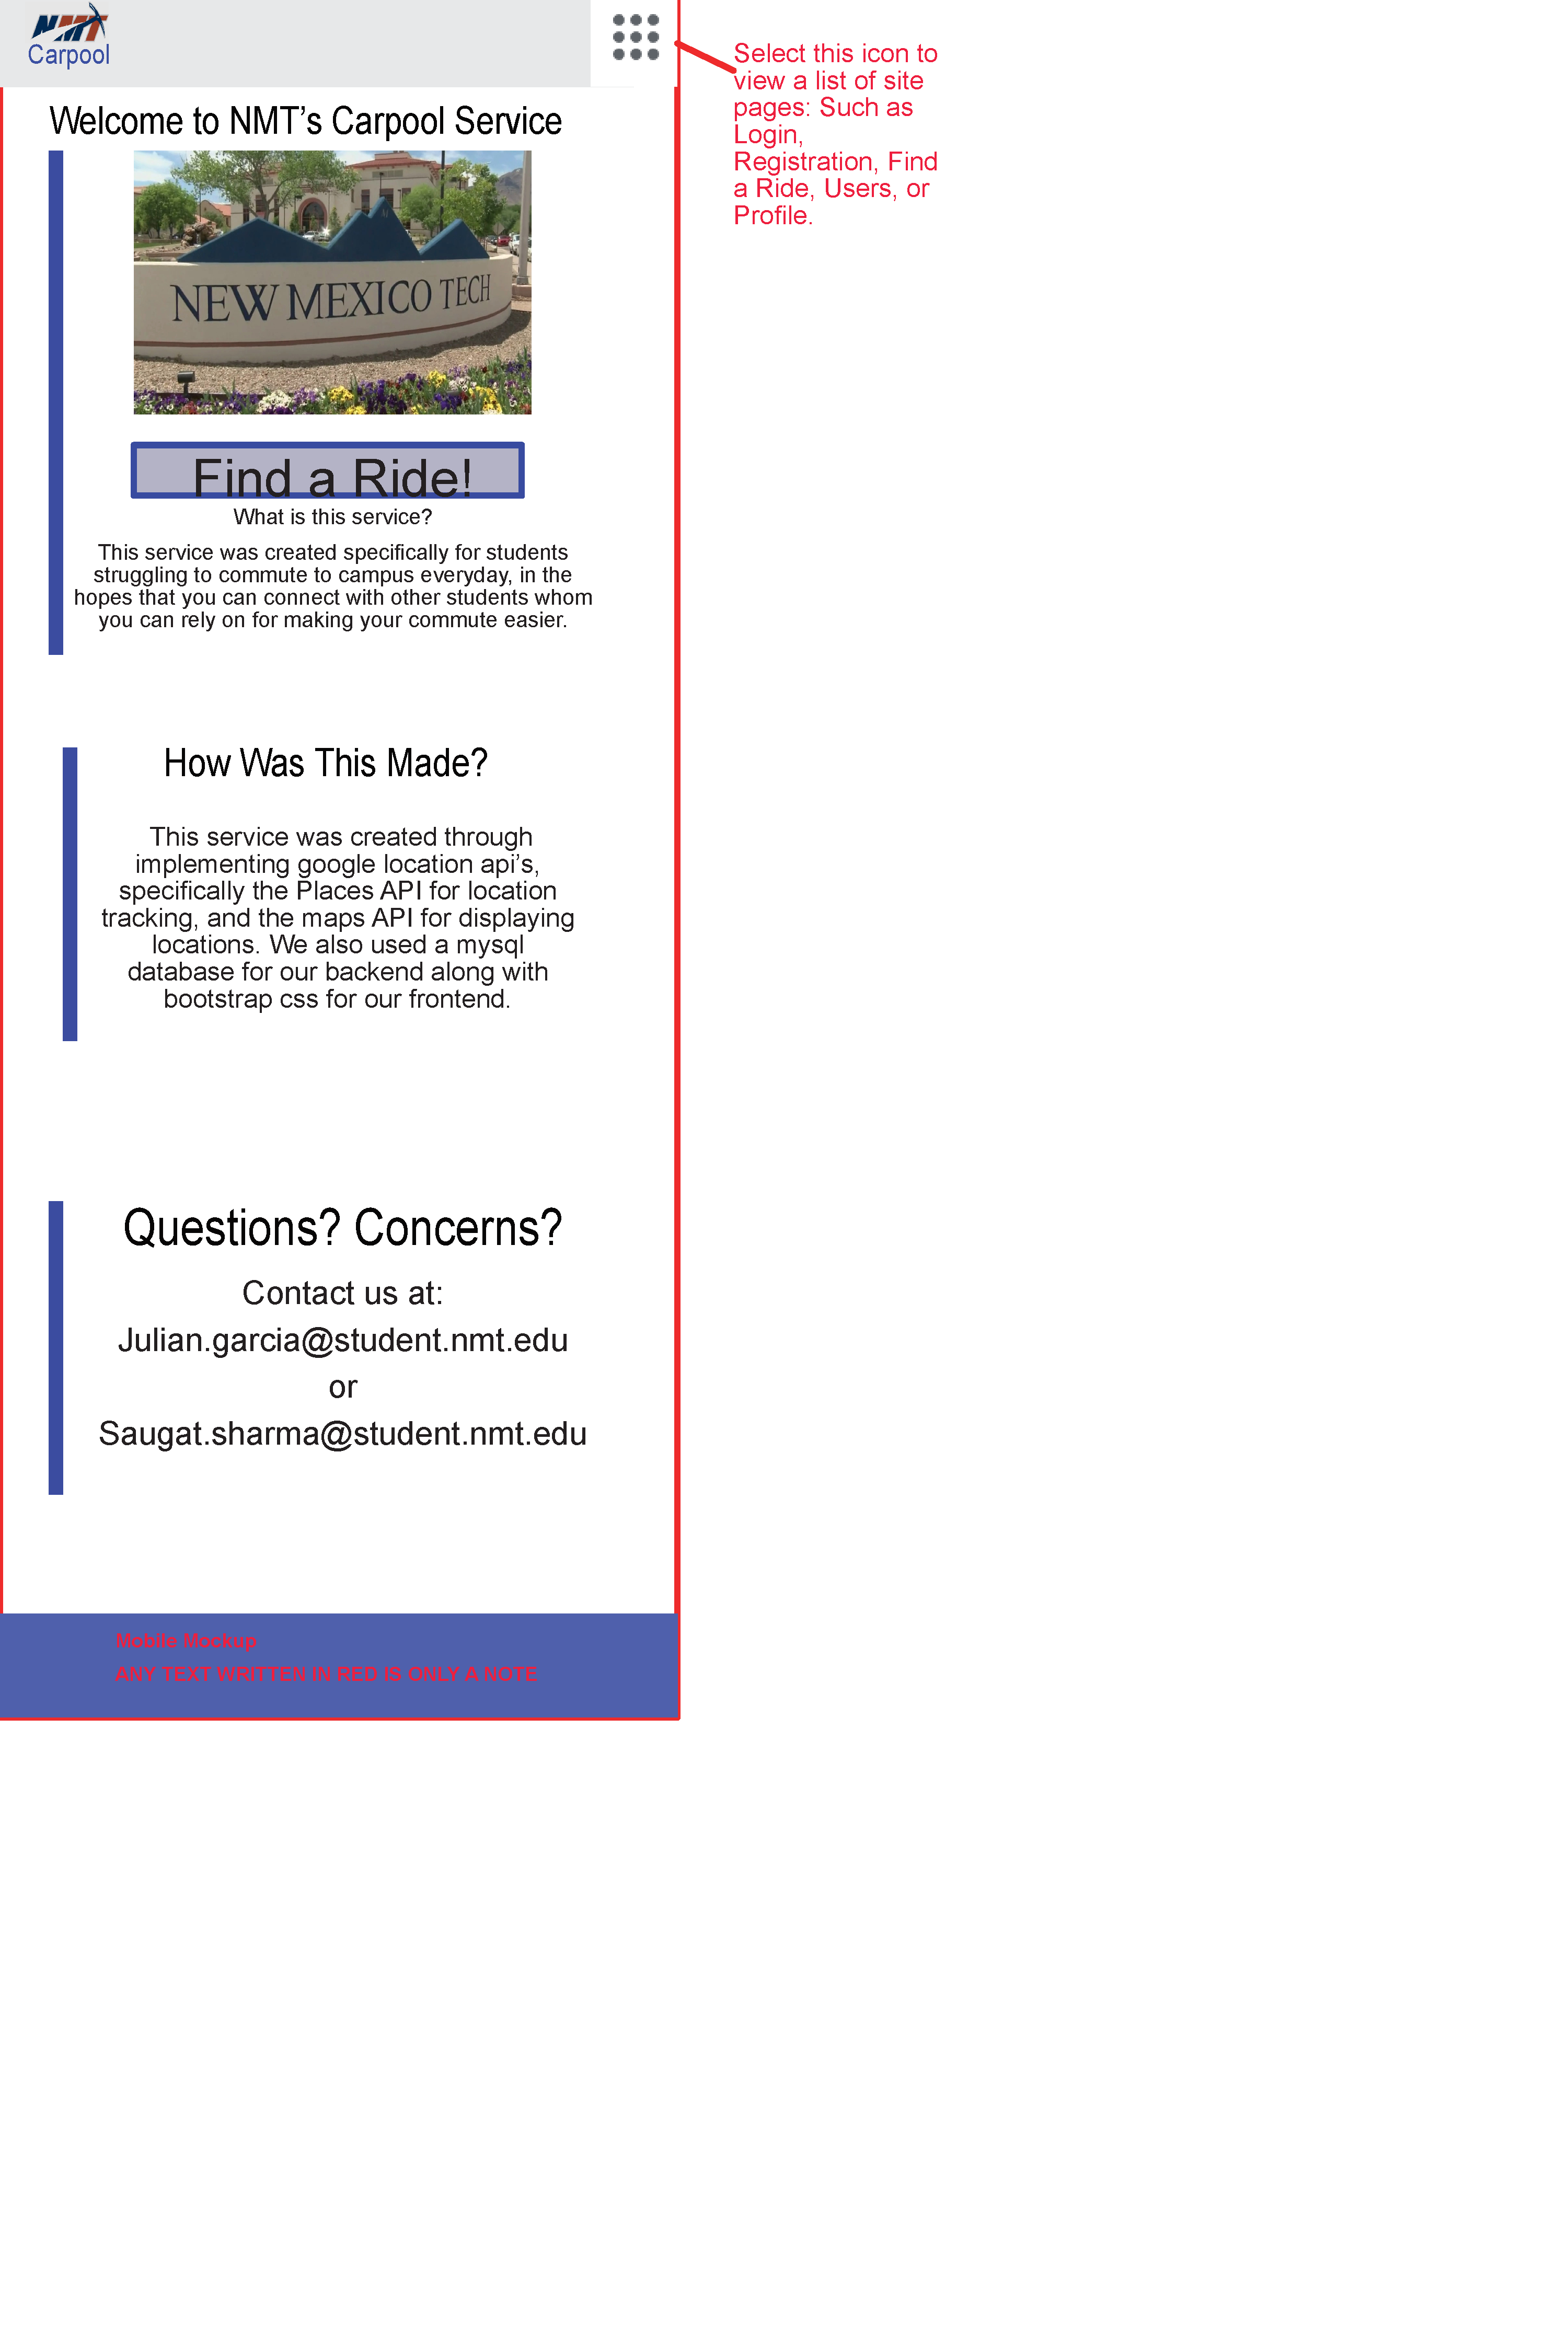
\includepdf[pages={-}]{MobileMockup.pdf}

\end{document}
